\section{\acf{SDL}}
\label{sc:SDL}
Die \acs{SDL} (\ac{SDL}, engl. Spezifikations und Beschreibungssprache) ist eine von der \ac{ITU-T} (\ac{ITU-T}, engl. Internationalen 
Telekommunikations- Vereinigung für Standardisierung der Telekommunikation) standardisierte objektorientierte Modellierungssprache und die erste Version wurde erstmalig 
1976 definiert. Die aktuellste Version von \ac{SDL} ist \ac{SDL}-2010 aus dem Jahre 2007, welche eine Überarbeitung der \ac{SDL}-Version \ac{SDL}-2000 aus dem Jahre 
1999 ist \cite[vii,51]{ITUT100_2016}. Wenn im folgenden von \ac{SDL} gesprochen wird, wird immer die Version \acs{SDL}-2010 gemeint. 
\ac{SDL} wird zur Beschreibung von Telekommunikationssystemen, deren Abläufe, sowie für Protokoll Definitionen und in verteilten Systemen eingesetzt.
Der Anwendungsbereich erstreckt sich über komplexe ereignisgesteuerte, interaktiven Echtzeitanwendungen, welche über Nachrichten miteinander kommunizieren. 
Der Hauptfokus von \ac{SDL} ist, sich einen genauen Überblick über das Verhalten genannter Systeme zu machen, wobei Eigenschaften mit anderen Techniken beschrieben werden müssen \cite[1\psq]{ITUT100_2016}. 
So wird \ac{MSC} unter anderem zum Beschreiben von Interaktionsverhalten zwischen Systemen, \ac{ASN1} für die Beschreibung von Datentypen und \ac{TTCN3} für Tests verwendet. In den letzten Überarbeitungen wurde die Spezifikation von \ac{SDL} um objekt-orientierte Aspekte erweitert und mit Sprachen wie \ac{UML} und \ac{ASN1} harmonisiert \cite[vii\psqq]{ITUT100_2016}. \ac{SDL} kann entweder grafisch oder textuell beschrieben werden. Beide Notationen sind semantisch äquivalent und lassen sich ineinander überführen \cite[3]{Weber_2008}.

\subsection{Architektur}
\label{ssc:Architektur}
Die \ac{SDL}-Spezifikation beschreibt ein hierarchisches System und erlaubt die strukturierte Trennung in Diagramme und Pakete und somit ein aufteilen eines Systems in viele kleinere Teilsysteme. Dies wirkt sich positiv auf die Entwicklung eines Systems in größeren Gruppen aus und vereinfacht diese. Ein System ist eine Menge an Blöcken, welche über Kanäle miteinander und der Umgebung außerhalb des Systems verbunden sind. Ein Kanal besitzt die Namen der Nachrichten bzw. Signale, welche über ihn übertragen werden können. Blöcke können Mengen von weiteren Blöcken enthalten oder als Prozess verfeinert dargestellt werden. Ebenso können Prozesse eine Menge von Prozessen in sich definiert haben.
Ein Prozess ist auf der untersten hierarchischen Ebene und beschreibt das dynamische Systemverhalten. Dies wird durch endliche Automaten, den \ac{EFSM} um genauer zu sein, beschrieben. Diese besitzen abstrakte Datentypen und Merkmale von Objektorientierung \cite[3\psq]{ITUT100_2016}. Diese Strukturhierarchie wird anhand folgender Abbildung \ref{fig:Agenten} veranschaulicht.
 
\begin{figure}[h]
	\centering
	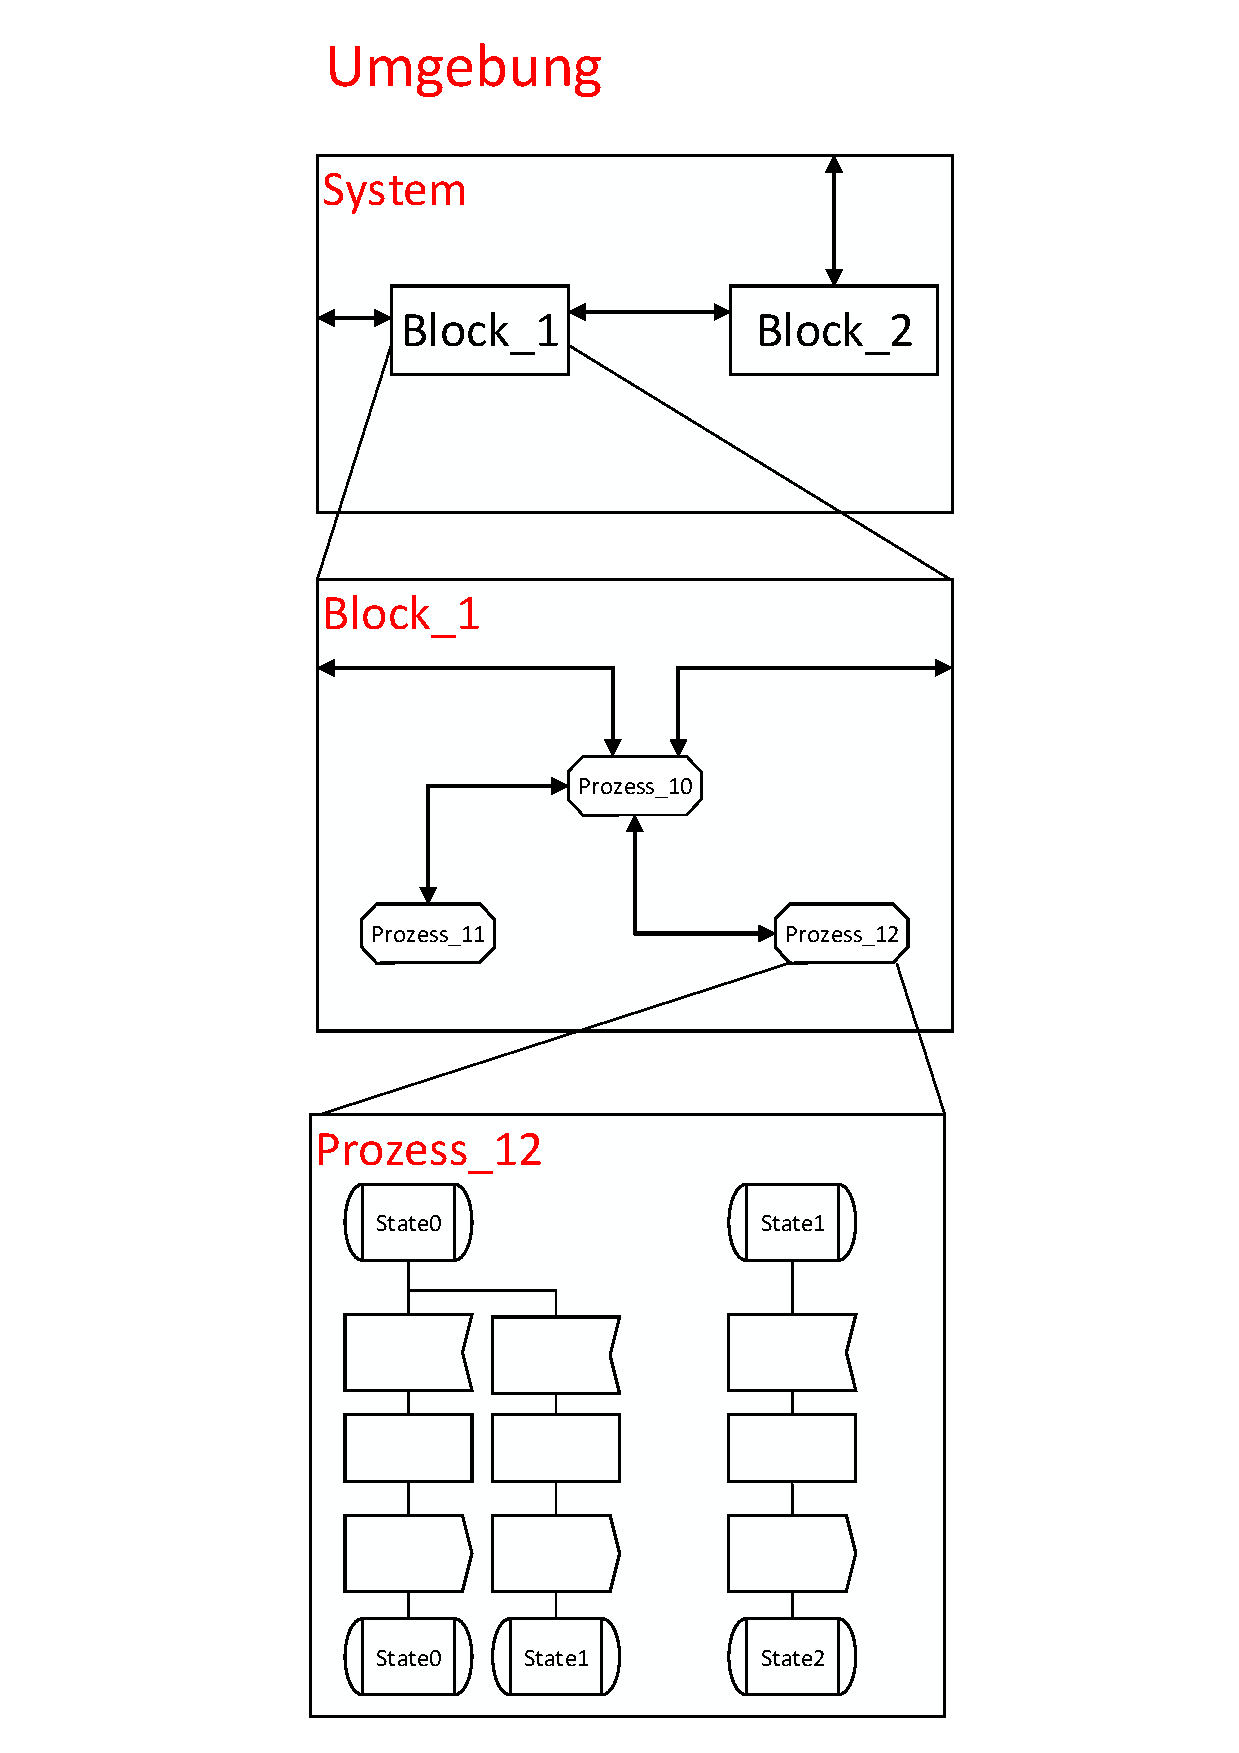
\includegraphics[width=1\textwidth]{Graphics/Agenten.pdf}
	\caption{SDL Architekturhierarchie}
	\label{fig:Agenten}
\end{figure}

\subsubsection{Agenten}
Seit \ac{SDL}-2000 werden alle Funktionsblöcke übergreifend als Agenten bezeichnet. Der System-Agent, ist ein speziell ausgezeichneter Block-Agent. Er beinhaltet weitere Block-Agenten und definiert die Nachrichten mit denen über die Umgebung kommuniziert wird. Block- und Prozess-Agenten unterscheiden sich in über die Kontrolle ihrer Ausführungsart. Wo die Zustandsmaschinen von Block-Agenten nebenläufig ablaufen können, müssen Prozess-Agenten auf den Abschluss der in Ausführung befindlichen Transaktion warten um ihren Zustand wechseln zu können \cite[29\psq]{ITUT101_2016}.


\subsection{Kommunikation}
\label{ssc:Kommunikation}
Die Kommunikation innerhalb von \ac{SDL} findet asynchron über Nachrichten bzw. mit diskreten Signalen (in \ac{SDL} signals) über Kanäle (in \ac{SDL} channel) statt. 
Diese können sowohl auf Systemebene, als auch auf Blockebene definiert werden und verbinden die Agenten untereinander oder mit der Umgebung.
Jeder Kanal besitzt einen Namen, genauso wie Nachricht aber auch optionale Parameter besitzen und in eine Liste gruppiert werden können.
Ein Kanal besteht immer aus einer Quelle und einem Endpunkt. Kanäle werden entweder Bi- oder Unidirektional definiert. Der Kanal muss entweder in einem anderen Agenten oder in die Umgebung (in \ac{SDL} environment) enden. Er kann aber auch den innerbefindlichen Prozess eines Agenten mit der Umgebung bzw. mit einem anderen innerbefindlichen Agenten verbinden \cite[39-42]{ITUT101_2016}. Dabei ist die Umgebung alles, was in einer \ac{SDL} spezifischen Sprache mit dem System kommunizieren kann \cite[3\psq]{ITUT100_2016}.
Abbildung \ref{fig:KommModell} verdeutlicht dies in einem Beispiel.
 
\begin{figure}[ht]
	\centering
	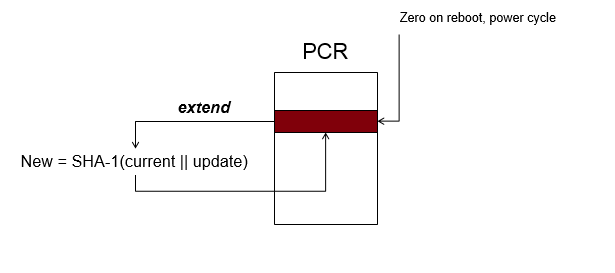
\includegraphics[width=1\textwidth]{test.png}
	\caption{Kommunikationsmodell}
	\label{fig:KommModell}
\end{figure}

\subsection{Systemverhalten}
\label{ssc:Verhalten}
Das Verhalten von \ac{SDL} wird in Prozessen definiert, welche automatenbasiert und wie eben besprochen, mittels \ac{EFSM}s repräsentiert werden. Sie bestehen aus einer Menge an Zustandsübergängen, welche Beispielhaft in Abbildung \ref{fig:Basiskonstrukte} zu sehen sind. Darunter gehören Zustände wie Start, Bedingung, Eingabe und Ausgabe. Da eine Aufzählung dem Sinn der Arbeit nicht dienlich ist, wird in diesem Zusammenhang auf die Spezifikation verwiesen \cite[44 \psqq]{ITUT101_2016}.
Ein Prozess besitzt eine Prozess-Id (in \ac{SDL} PId), damit bei Instanziierung eines Prozesses, diese unterschieden werden können. Zusätzlich besitzt er einen Eingabepuffer zum Speichern von Nachrichten. Dieser Puffer übergibt nach dem \ac{FIFO}-Prinzip nacheinander die anstehenden Nachrichten des verbundenen Kanals an den Prozess \cite[42]{ITUT101_2016}. Kommen zwei Nachrichten von mehreren Kanälen gleichzeitig an einem Prozess an, so ist das Systemverhalten undefiniert und nach dem Zufall wird eine der beiden Nachrichten zuerst ausgeführt.
Die Modellierung der Automaten richtet sich oft nach Mealy, wobei in diesem die Ausgabe von seinem Zustand und seiner Eingabe abhängt.
Im Gegensatz zu Moore-Automaten enthält er keinen Startzustand, wobei jeder Mealy-Automat in einen Moore-Automat übertragen werden kann.


\begin{figure}[h]
	\centering
	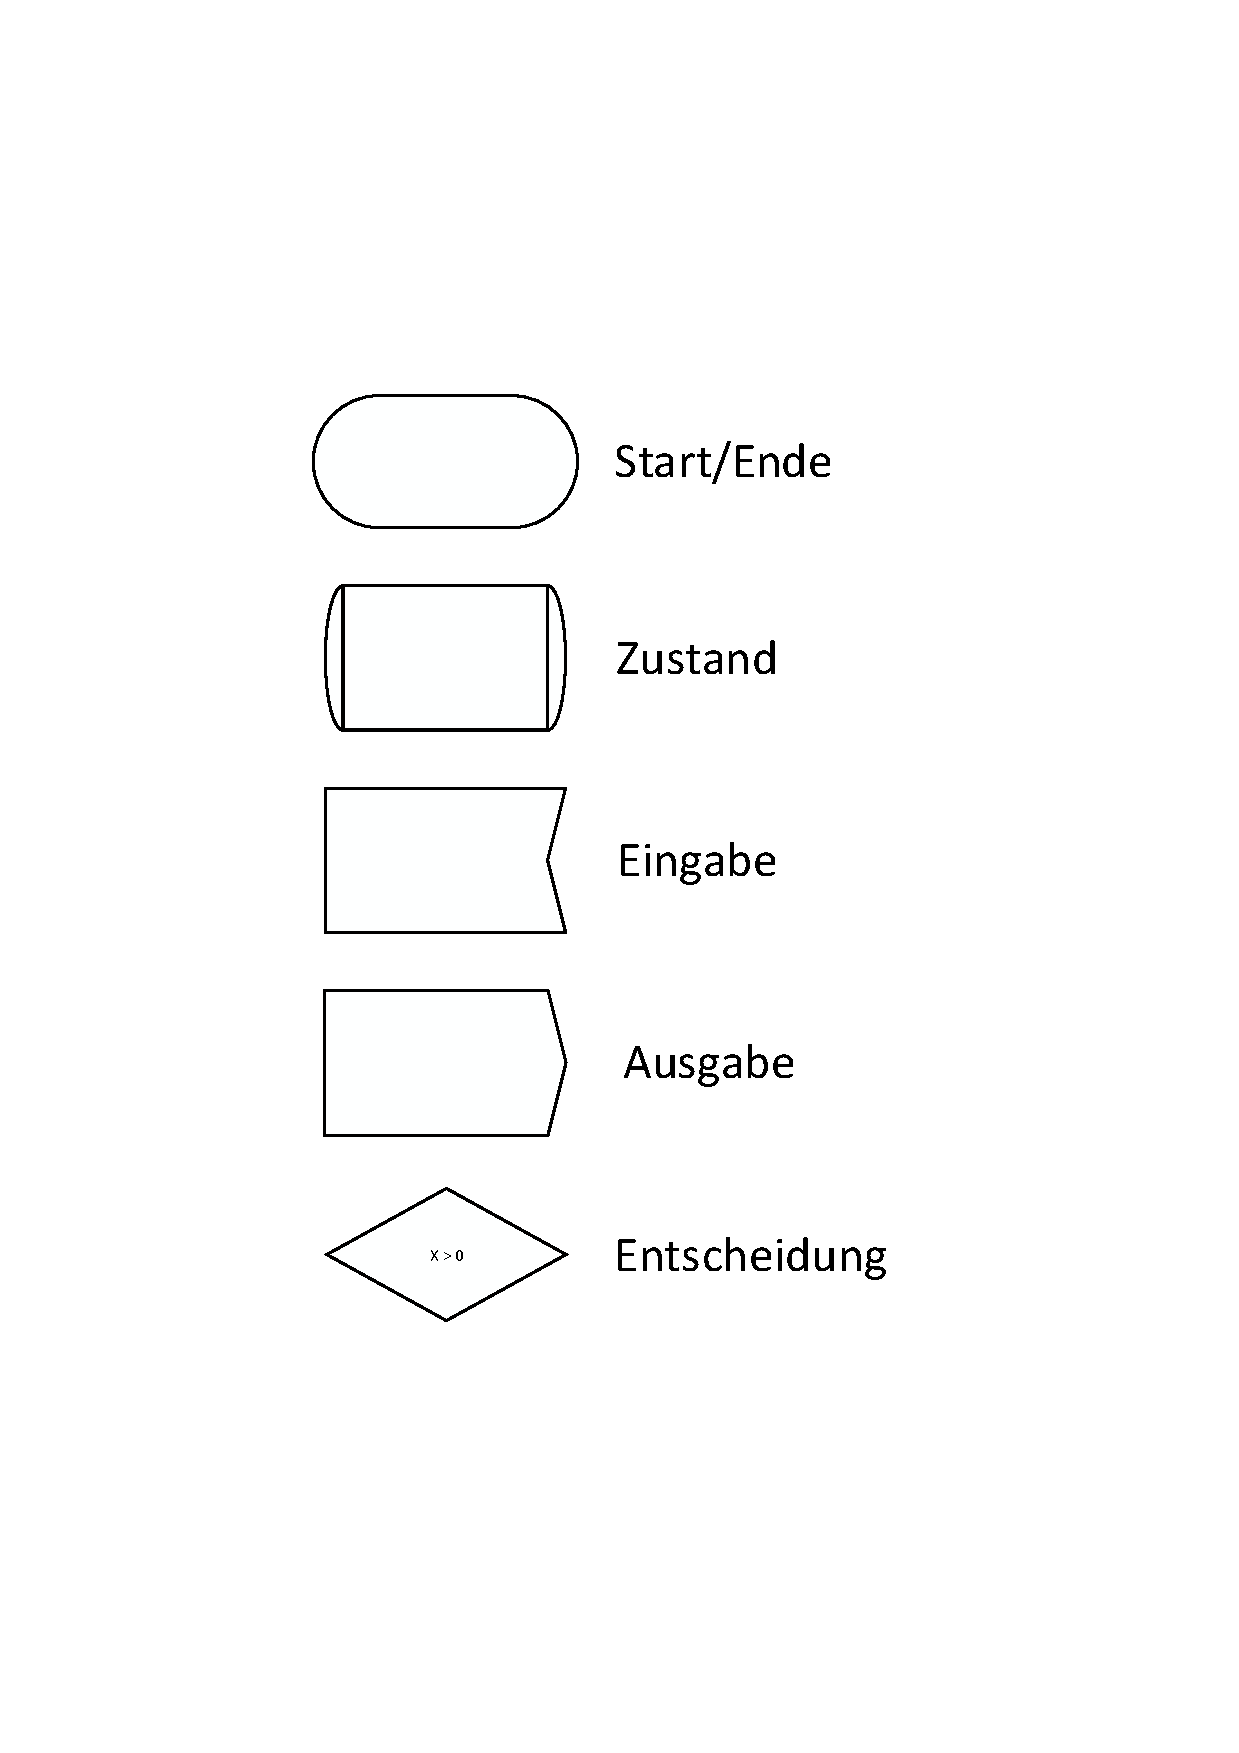
\includegraphics[width=0.5\textwidth]{Graphics/Basiskonstrukte.pdf}
	\caption{SDL-Basiskonstrukte}
	\label{fig:Basiskonstrukte}
\end{figure}v


\subsection{Datenmodellierung}
\label{ssc:Daten}
In \ac{SDL} können Daten auf zwei Arten beschrieben werden, einerseits mit dem \acs{ADT} oder mit \ac{ASN1}. \ac{ADT} definiert keine Datenstrukturen, sondern jeweils einen Satz (in \ac{SDL} sorts) an Werten, Operation und Bedingungen \cite[67]{ITUT104_2016}. In \ac{ADT} sind einige Datentypen wie Boolean, Character, Charstring, Integer und Real vordefiniert, aber auch Konstrukte wie Array und Enum. Eine Liste der vordefinierten Datentypen kann aus der Spezifikation entnommen werden \cite[47\psqq]{ITUT104_2016}. Neue Datentypen lassen sich durch bereits vorhandene Datentypen definieren, hierzu sind Einschränkungen und ein Standardwert in der Definition mit anzugeben. Abbildung \ref{fig:DatentypDef} verdeutlicht dies in einem Beispiel. In jedem Agenten lassen sich Konstanten, basierend auf den gewählten Datentypen definieren. Sie müssen einen konstanten Wert enthalten und dürfen nicht verändert werden. Variablen können nur in Prozessen definiert werden, enthalten denselben Aufbau wie Konstanten und können nur in ihrem definierten Prozess geändert werden. Zwar sind keine globalen Variablen zulässig, jedoch können Prozess eigene Variablen anderen Prozessen sichtbar gemacht werden. Diese Variablen nennt man remote variables \cite[31]{ITUT102_2016}.


\begin{figure}[h]
	\centering
	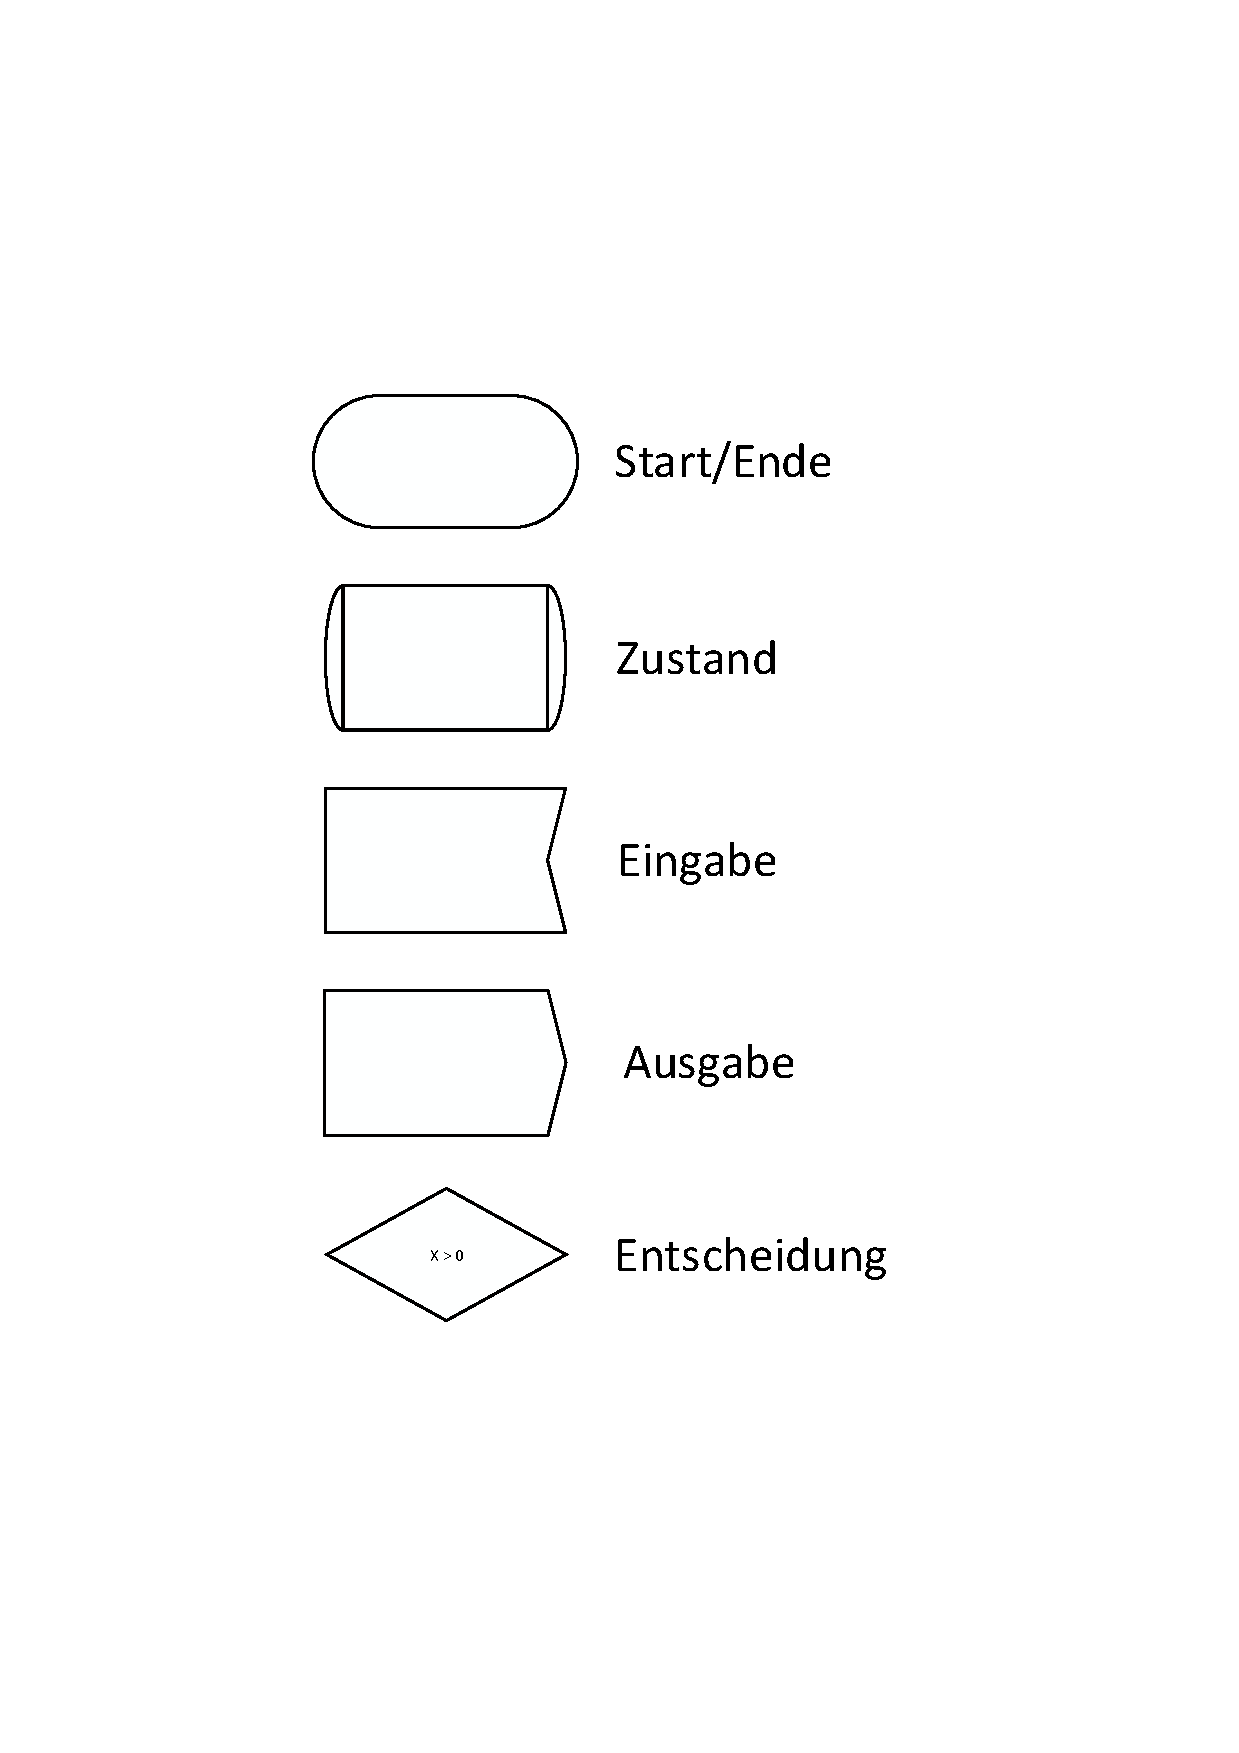
\includegraphics[width=0.5\textwidth]{Graphics/Basiskonstrukte.pdf}
	\caption{SDL-Datentypdefinition}
	\label{fig:DatentypDef}
\end{figure}v


\begin{figure}[h]
	\centering
	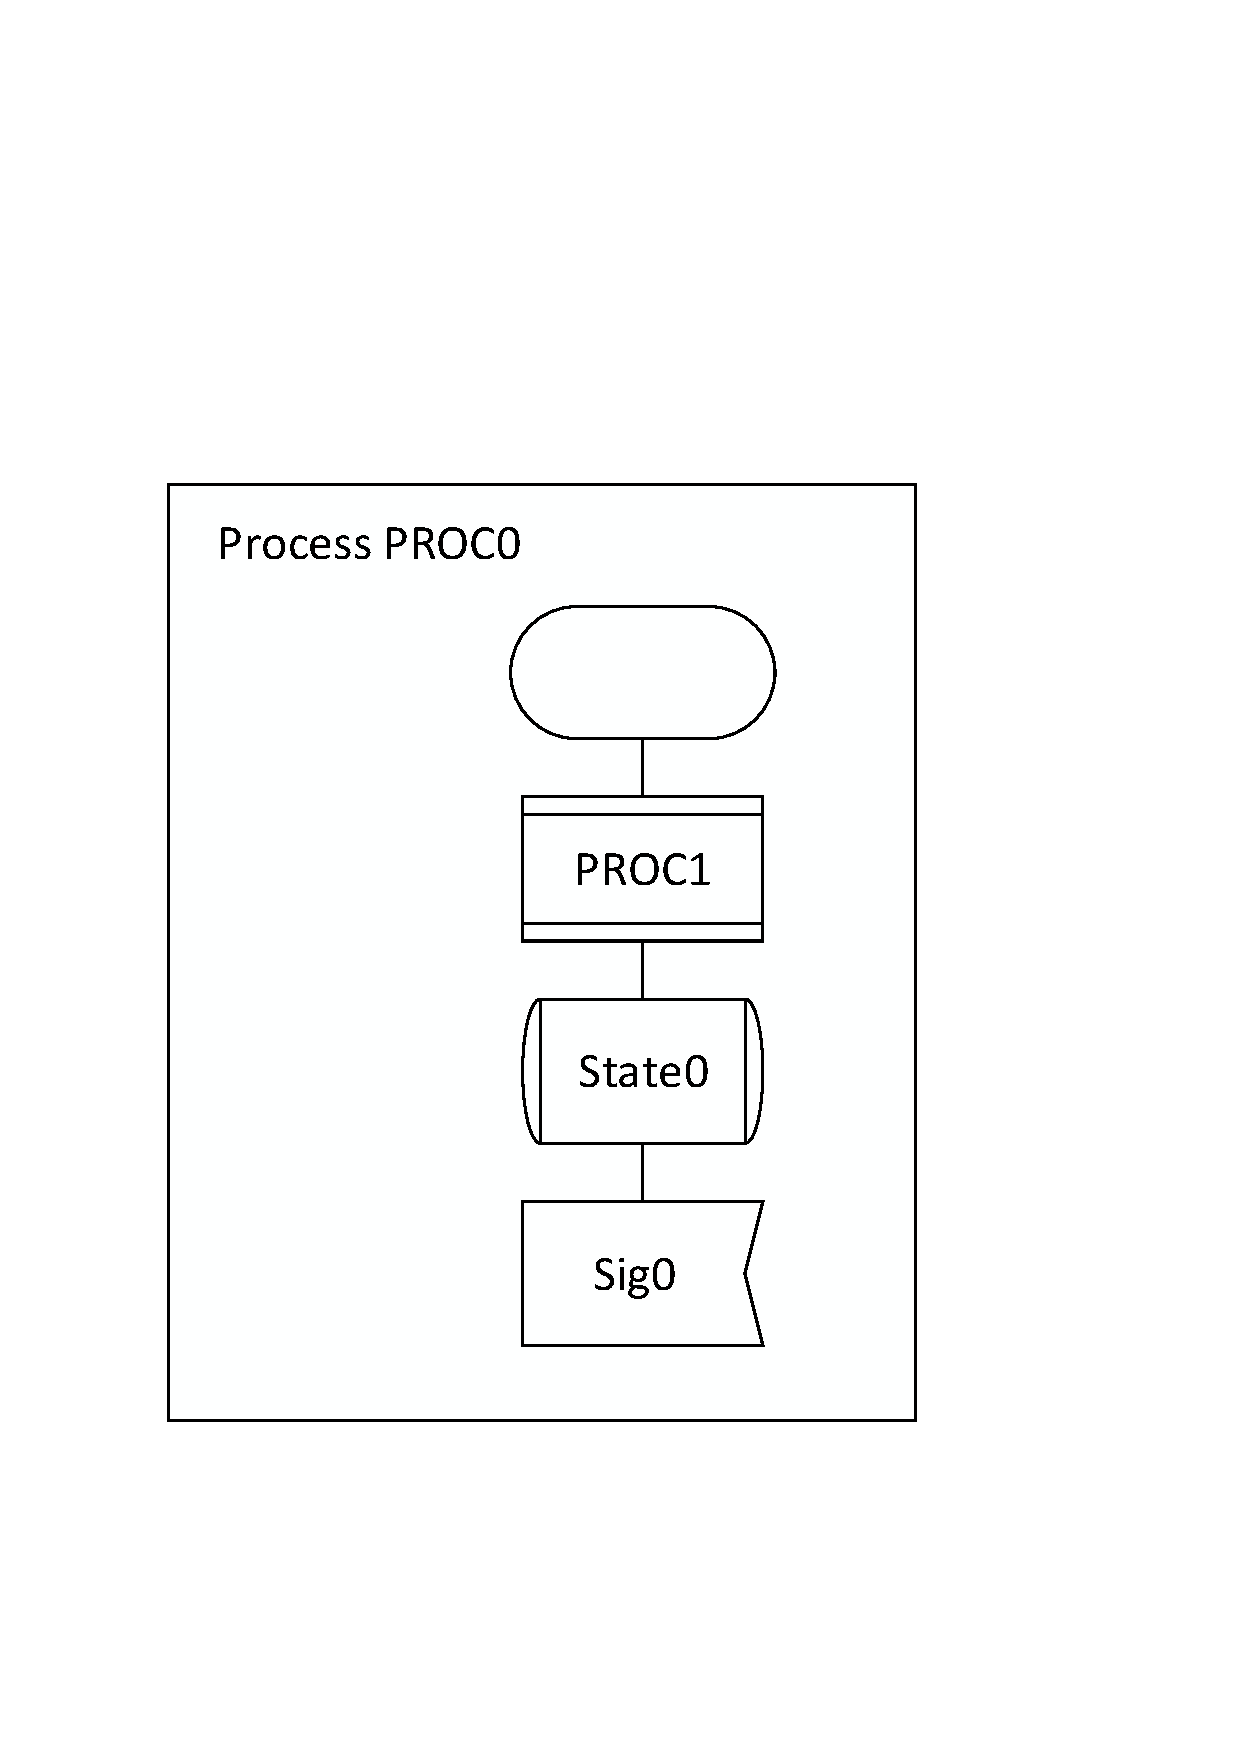
\includegraphics[width=0.5\textwidth]{Graphics/ProcessInit.pdf}
	\caption{SDL-Prozessinitialisierung}
	\label{fig:ProcessInit}
\end{figure}v


\subsection{Objektorientierung} 
\label{ssc:Vererbung}
Die objektorientierten Konzepte von \ac{SDL} bieten dem Anwender eine Möglichkeit sein System zu strukturieren, wiederzuverwenden und das Modell ähnlicher der Realwelt abzubilden. So ist es möglich für einen Prozess-/Block-Agenten eine Prozess-/Block-Klasse zu erstellen. Im objektorientierten Ansatz werden diese auch als Typ (in \ac{SDL} type) bezeichnet. Diese werden für die Instanziierung, Vererbung und Spezialisierung von Typen verwendet. Ein Klassenagent kann auf jeder beliebigen Ebene definiert werden, egal ob nahe beim Kontext oder nicht.
Bei der Verwendung von Klassen, unterscheiden sich der objektorientierte und nicht-objektorientierte Ansatz syntaktisch zuerst nicht. Jedoch ist es möglich im objektorientierten Ansatz Instanzen der Klasse zu erzeugen \cite[4\psqq]{ITUT100_2016}.


\begin{figure}[h]
	\centering
	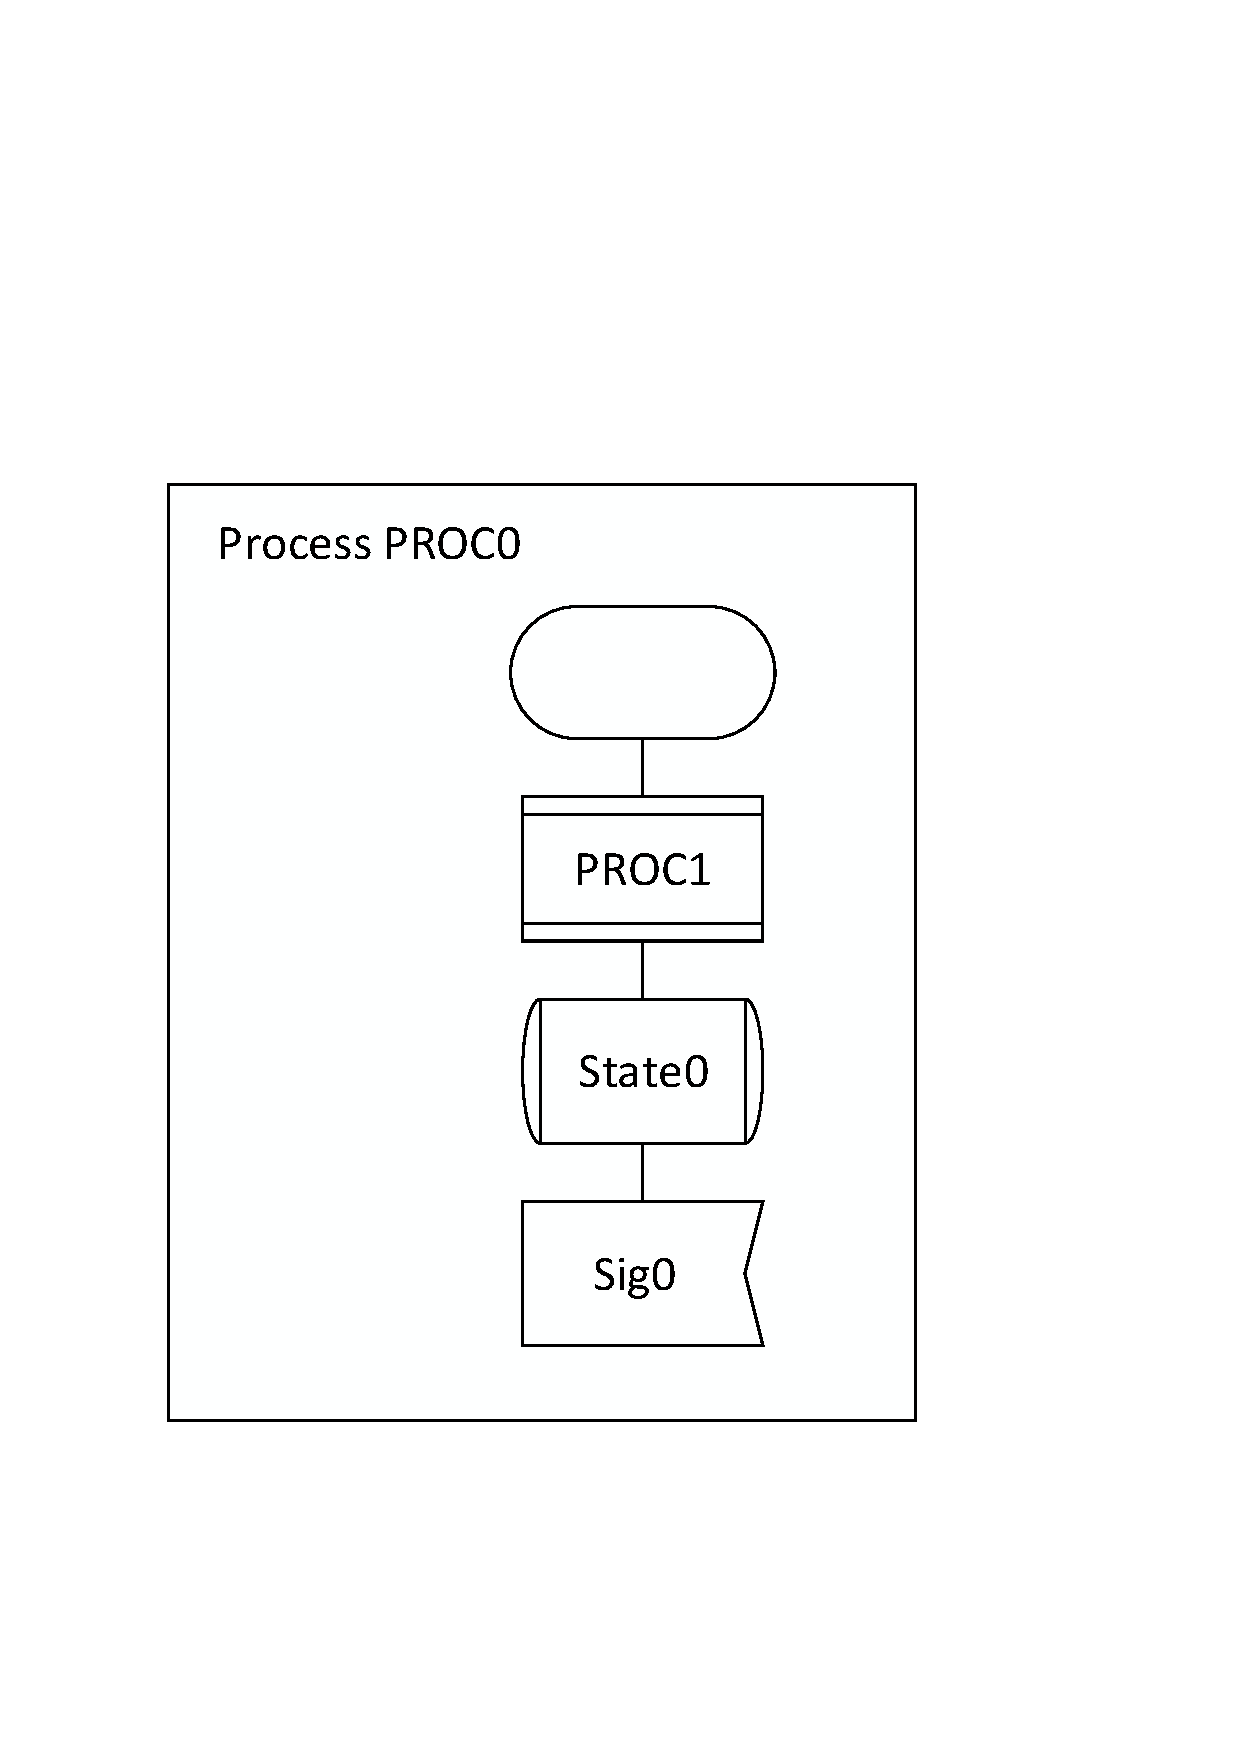
\includegraphics[width=0.5\textwidth]{Graphics/ProcessInit.pdf}
	\caption{OO-Konzepte von SDL}
	\label{fig:OOKonzept}
\end{figure}v

\subsection{Spracheigenschaften}
\label{ssc:Spracheigenschaften}
Die Eigenschaften der Sprachdefinition von \ac{SDL} sind folgend beschrieben\cite[2\psq]{ITUT111_2016}:
\begin{itemize}{
		\item[Abstrakte Grammatik] Die abstrakte Grammatik von \ac{SDL} wird von einer abstrakten Syntax und statischen Bedingungen 
		beschrieben. Die Abstrakte Syntax kann entweder mit einer textbasierten Grammatik oder einem grafischen Metamodell erstellt werden.
		
		\item[Konkrete Grammatik] Die konkrete Grammatik wird durch eine grafische Syntax, statischen Bedingungen und Regeln für die grafische Syntax beschrieben.
		Beschrieben wird sie durch die erweiterte Backus-Naur Form. Wenn jedoch in der abstrakten Grammatik ein 
		grafisches Metamodell verwendet wurde, ist es erlaubt dieses um konkrete Eigenschaften zu erweitert und zu verwenden.
		
		\item[Semantik] Die Semantik gibt einem Konstrukt eine klare Bedeutung. Sie enthält dessen Eigenschaften, die Art der Interpretation und dynamischen Bedingungen die erfüllt sein müssen, damit das Konstrukt sich so verhält, sodass es in der Art verhält wie die Sprache gestaltet wurde. Die Eigenschaften sind wohl definierte Beziehungen, zwischen verschiedenen Konzepten.
		
		\item[Model] Das Model gibt Notationen eine Abbildungsform, wenn diese keine direkte abstrakten Syntax besitzen. Diese sind dann nach der konkreten Syntax anderer Konstrukte zu modellieren. Diese Konstrukte werden als "shorthand" bezeichnet und  beinhalten die Syntax der transformierten Form.
}\end{itemize}

\subsubsection{Metamodell}
\label{ssc:Metamodell}
Es werden derzeit Anstrengungen unternommen ein öffentlich zugängliches Metamodell von \ac{SDL} zu erstellen, welches alle Aspekte der Sprache in sich vereinigt. Zu dem derzeitigen Standpunkt existiert jedoch keines oder ist nicht uns bekannt. Deswegen hat die \ac{ITU-T} selbst ein Meta-Metamodell auf Grundlage von 
\ac{UML} erstellst, welches jedoch auch die Definition nicht vollends abdeckt. Das Meta-Metamodell wird auch als SDL-UML bezeichnet \cite[18]{ITUT109_2016}.
